\chapter{Validation}
\label{chap:validation}

\section{Introduction}
This chapter unfolds as a meticulous exploration into the performance and reliability of the Fair-by-Design workflow. To conduct a thorough assessment, the Educational Dataset obtained by ULL has been strategically chosen as the testing ground. This dataset, rich in attributes that can be both protected and impactful on students' performance in a specific subject, provides a nuanced platform for evaluating the workflow's effectiveness across various machine learning algorithms.

The central emphasis of this validation endeavor is to ascertain not only the accuracy and predictive capabilities of the implemented models but also the extent to which the Fair-by-Design workflow succeeds in fostering fairness. The Educational Dataset allows for a detailed examination of how different algorithms respond to the intricacies of real-world educational data, shedding light on the interplay between accuracy and fairness.

Throughout this chapter, the validation process unfolds systematically, encompassing diverse algorithms applied to the Educational Dataset. The goal is to detect both the strengths and potential limitations of the Fair-by-Design approach, providing valuable insights for its application in educational scenarios where the equitable treatment of students and the accuracy of predictions are of paramount importance. The subsequent sections detail the experimental setup, algorithmic choices, and the rigorous evaluation metrics employed to ensure a comprehensive understanding of the Fair-by-Design workflow's performance on the chosen educational dataset.

\section{Dataset description}

Before delving into the intricate details of the algorithm implementations presented earlier, it is imperative to provide a comprehensive overview of the dataset on which these algorithms have been applied. The chosen dataset for this work is the \emph{Canary Island Educational dataset}, an invaluable resource that underpins the empirical exploration of bias mitigation strategies in the context of the educational system in the Canary Islands. 

The Canary Island Educational dataset is a rich and expansive repository of information, meticulously compiled to capture various facets of the educational landscape within the Canary Islands. This dataset comprises the comprehensive census of students enrolled over four distinct academic years, offering a multifaceted glimpse into the educational ecosystem. 

The dataset encompasses a diverse array of attributes and data points, encapsulating critical information such as student demographics, academic performance, socioeconomic factors, and other pertinent variables. These attributes collectively provide a holistic perspective on the educational landscape, enabling a nuanced analysis of the factors that influence student outcomes and experiences. 

The temporal dimension of the dataset, spanning four academic years, further enriches the analytical potential. It allows for the investigation of temporal trends, shifts in educational policies, and the evolution of student characteristics over time. This temporal depth is particularly valuable when examining the efficacy of bias mitigation strategies, as it facilitates the assessment of their impact across different academic years. 

The Canary Island Educational dataset is not merely a repository of numbers and statistics; it is a window into the educational opportunities and challenges faced by students in the Canary Islands. By harnessing the insights gleaned from this dataset, it becomes possible to proactively address biases and promote equity within the educational system, ultimately striving for a more inclusive and just educational landscape.

\section{Precise Definition of Objectives}
\label{section:val_obj}

In this section, are meticulously outlined the objectives that intricately guide the Fair-by-Design workflow, with a primary focus on achieving effective prediction about the english level of each student while concurrently addressing fairness considerations and mitigating biases. The critical components encompass the meticulous identification of protected attributes, the strategic selection of fairness notions, and the corresponding choice of fairness metrics.

\subsection{Prediction Objective}

The overarching objective is to execute a fairness-driven classification task, discerning whether a student's english level is either above or under a certain threshold for each student enrolled in the 4 grade.

\subsection{Protected Attributes}

The identified protected attributes for scrutiny within the Fair-by-Design framework are the following:

\begin{itemize}

    \item sex

    \item capital island: if the student comes from the capital of the city

    \item public\textunderscore private: if the school is public or private
    
    \item mothly houseold income

    \item economic, social and cultural satus index

\end{itemize}

These attributes hold particular significance in the context of potential biases and fairness considerations.

\subsection{Fairness Notions}

To operationalize fairness, two distinct notions are employed, each serving specific objectives:

\begin{itemize}
    \item \emph{Demographic Parity:} The objective is to ensure a consistent distribution of predicted outcomes across different subgroups delineated by the protected attributes. This aligns with the broader goal of fostering equity in predictions.

    \item \emph{Group Fairness:} The goal is to guarantee equitable predictions within specific subgroups defined by protected attributes. This notion emphasizes the need for fairness at a more granular level, considering distinct demographic categories.
\end{itemize}

\subsection{Fairness Metrics}

To quantify and assess fairness in the context of the defined notions, specific fairness metrics are employed:

\begin{itemize}
    \item \emph{For Demographic Parity:} The chosen metric is \emph{Disparate Impact}, offering a quantitative measure of the disparate outcomes across different subgroups.

    \item \emph{For Group Fairness:} The metric utilized is \emph{Demographic Parity Difference}, providing a nuanced assessment of fairness within specific demographic subgroups.
\end{itemize}

These meticulously defined objectives, coupled with the chosen fairness notions and metrics, collectively establish a robust foundation for the Fair-by-Design workflow. This ensures a focused approach towards accurate predictions while concurrently fostering fairness and equity across diverse subgroups.

\section{Data Collection Details}
\label{section:val_dc}

In this section, we delve into the specifics of the data collection process, providing a comprehensive overview of the dataset and its division into distinct training and test sets.

\subsection{Dataset Overview}

The dataset comprises two distinct sets:

\begin{itemize}
    \item \emph{Training Set:} Consisting of 9,831 items and 100 attributes.
    \item \emph{Test Set:} Comprising 3,246 items and 100 attributes.
\end{itemize}

\subsection{Dataset Composition}

The dataset encompasses 99 independent features of diverse types, each contributing valuable information for predictive modeling. Additionally, there is one dependent variable, representing whether a student's english level is beyond or above a certain threshold. Each record within the dataset corresponds to an individual, and the output variable is binary, delineating income categories.

\subsection{Protected Attributes and Encoding Consistency}

As identified in \cref{section:val_obj}, five discrete protected attributes play a crucial role in fairness considerations. It is imperative to note that these attributes are discrete in nature. Furthermore, an essential consideration for subsequent analyses pertains to the representation of the output variable. Although it is binary, it is currently encoded as a string. Ensuring consistency in the encoding of this variable across both the training and test sets is of paramount importance for accurate and meaningful analyses in subsequent stages.

This detailed understanding of the dataset's composition and attributes provides a solid foundation for subsequent steps in the Fair-by-Design workflow, facilitating informed decisions regarding model development and fairness considerations.

\section{Data pre-processing}

Starting from the information provided by \cref{section:val_dc} in this section all the variables represend as string as been labeled the same manner. This led to a consistent dataset to be used in the models training.

\section{Algorithm design}
\label{section:val_alg}

In the context of the Fair-by-Design workflow, four key fairness algorithms have been strategically chosen to comprehensively test the workflow's effectiveness. Each algorithm serves a specific purpose within the workflow, contributing to the overarching goal of achieving fairness in predictions.

\subsection{Pre-processing Algorithms}

\subsubsection{Data Augmentation Algorithm}

\begin{itemize}

    \item \emph{Algorithm Description:} The proposed data augmentation algorithm introduces synthetic samples to the training dataset. By augmenting the data, especially focusing on underrepresented groups, the algorithm aims to enhance the model's exposure to diverse scenarios, promoting a more robust understanding of the underlying patterns.

    \item \emph{Reasoning:} Data augmentation is crucial for addressing imbalances in the training data, allowing the model to generalize better across different groups and mitigating biases stemming from insufficient representation.

\end{itemize}

\subsubsection{Fairness Through Unawareness}

\begin{itemize}

    \item \emph{Algorithm Description:} Fairness through unawareness involves deliberately avoiding the use of sensitive attributes in the modeling process. This pre-processing approach aims to promote fairness by excluding potentially biased features, thus reducing the risk of discrimination based on sensitive attributes.

    \item \emph{Reasoning:} Fairness through unawareness is considered to mitigate biases by preventing the model from directly using sensitive attributes, thereby minimizing the potential for biased predictions associated with these attributes.

\end{itemize}

\subsection{In-processing Algorithms}

\subsubsection{ExponentiatedGradient}

\begin{itemize}

    \item \emph{Algorithm Description}: The ExponentiatedGradient algorithm applies iterative re-weighting to the training data, seeking to find a fair classifier by minimizing the disparity in predictions across sensitive groups.

    \item \emph{Reasoning:} ExponentiatedGradient is chosen for its versatility and effectiveness in in-processing fairness. It provides a fine-tuning mechanism during training to achieve parity in predicted outcomes.

\end{itemize}

\subsubsection{GridSearch}

\begin{itemize}

    \item \emph{Algorithm Description:} GridSearch is a generic algorithm that explores a range of hyperparameter values to find the optimal configuration for a fair classifier.

    \item \emph{Reasoning:} GridSearch is included to assess the impact of hyperparameter tuning on fairness outcomes, offering insights into the versatility of the approach.

\end{itemize}

The choice of these four algorithms is driven by the aim of obtaining a holistic view of the Fair-by-Design workflow's performance. By incorporating diverse pre-processing, in-processing, and post-processing strategies, the evaluation can capture the nuances of fairness considerations at different stages of the machine learning pipeline. This comprehensive approach ensures a thorough exploration of potential biases and fairness enhancements, laying the foundation for a robust and equitable model.

\section{Model training and evaluation}
\label{section:val_mt_eval}

\subsection{Model Training}

\subsubsection{Training Models}

The model training process involves the utilization of two distinct classifiers:

\begin{itemize}

    \item \emph{XGBoost}: XGBoost, an optimized gradient boosting algorithm, is selected for its ability to handle diverse datasets and deliver high predictive accuracy.

    \item \emph{RandomForest Classifier:} RandomForest classifier, known for its ensemble learning approach, is chosen to capture complex relationships in the data and enhance predictive performance.

\end{itemize}

subsection{Performance Evaluation}

\subsubsection{Results Evaluation}

The evaluation of general results encompasses an assessment of the overall model performance and the computation of fairness metrics.

It's important, before to provide a general view of the results, provide some considerations on the pre-processing algorithms:

\begin{itemize}
    \item \emph{Data augmentation}: this algorithm led the dataset from 9,831 to 83,028 items.
    \item \emph{Fairness through unawareness}: in order to apply this algorithm the protected attribute have been replaced with their \emph{median} value.
\end{itemize}

In order to provide a tabular representation of the results it's necessary to assign some labels to have a more compressed representation and two tables are reported, one for each metric:

\begin{itemize}
    \item \emph{Fairness algorithm}: FairAlg
    \begin{itemize}
        \item \emph{Data augmentation}: DA
        \item \emph{Fairness through unawareness}: FtU
        \item \emph{Exponentiated Gradient}: EG
        \item \emph{GridSearch}: GS
    \end{itemize}
    \item \emph{Model}
    \begin{itemize}
        \item \emph{XGB Classifier}: XGB
        \item \emph{RandomForest Classifier}: RF
    \end{itemize}
    \item \emph{Accuracy}: Acc
    \item \emph{Fairness metric}:
    \begin{itemize}
        \item Protected attribute: Sex
        \begin{itemize}
            \item \emph{Disparate Impact }: DIs
            \item \emph{Demographic Parity Difference}: DPDs
        \end{itemize}
        \item Protected attribute: Capital Island
        \begin{itemize}
            \item \emph{Disparate Impact }: DIc
            \item \emph{Demographic Parity Difference}: DPDc
        \end{itemize}
        \item Protected attribute: CPublic or Private school
        \begin{itemize}
            \item \emph{Disparate Impact }: DIp
            \item \emph{Demographic Parity Difference}: DPDp
        \end{itemize}
        \item Protected attribute: Household Income
        \begin{itemize}
            \item \emph{Disparate Impact }: DIh
            \item \emph{Demographic Parity Difference}: DPDh
        \end{itemize}
        \item Protected attribute: ESCS Index
        \begin{itemize}
            \item \emph{Disparate Impact }: DIe
            \item \emph{Demographic Parity Difference}: DPDe
        \end{itemize}
    \end{itemize}
\end{itemize}
\newpage
\textbf{Fairness metric: Disparate Impact}

\begin{figure}[H]
    \centering
    \begin{tabular}{|c|c|c|c|c|c|c|c|}
        \hline
        \textbf{FairAlg} & \textbf{Model} & \textbf{Acc} & \textbf{DIs} & \textbf{DIc} & \textbf{DIp} & \textbf{DIh} & \textbf{DIe} \\
        \hline
        DA & XGB & 0.9975 & 0.9670 & 0.9813 & 0.9901 & 0.9340 & 0.0007 \\
        \hline
        DA & RF & 0.9987 & 0.9670 & 0.9770 & 0.9901 & 0.8610 & 0.0013 \\
        \hline
        FtU & XGB & 0.9987 & 0.9750 & 0.9813 & 0.9942 & 0.8610 & 0.0019 \\
        \hline
        FtU & RF & 0.9987 & 0.9697 & 0.9770 & 0.9901 & 0.8610 & 0.0013 \\
        \hline
        EG & XGB & 0.9944 & 0.9779 & 0.9743 & 0.9919 & 0.8622 & 0.0019 \\
        \hline
        EG & RF & 0.9987 & 0.9697 & 0.9770 & 0.9901 & 0.8610 & 0.0013 \\
        \hline
        GS & XGB & 0.5201 & 0.0000 & 0.0000 & 0.0000 & 0.0000 & 0.0759 \\
        \hline
        GS & RF & 0.9987 & 0.9697 & 0.9770 & 0.9901 & 0.8610 & 0.0013 \\
        \hline
    \end{tabular}
    \caption{Models training results for disparate impact metric}
    \label{fig:results}
\end{figure}

About these results it's possible to make some consideration:

\begin{enumerate}

    \item For each model the metric for \emph{ESCS} is close to 0. This means that each algorithm the demographic parity is not achieved.

    \item On the other hand for every other protected attribute is close to 1, this means that for each algorithm, except the GridSearch, for these protected attributes, the demographic parity is achieved.

    \item The GridSearch algorithm with the XGB model completely fails into the achieving of the demographic parity, since the DI value is 0 for each protected attribute but \emph{ESCS}, for which it's close to 0.
    
\end{enumerate}

\newpage
\textbf{Fairness metric: Demographic Parity}

\begin{figure}[H]
    \centering
    \begin{tabular}{|c|c|c|c|c|c|c|c|}
        \hline
        \textbf{FairAlg} & \textbf{Model} & \textbf{Acc} & \textbf{DPDs} & \textbf{DPDc} & \textbf{DPDp} & \textbf{DPDh} & \textbf{DPDe} \\
        \hline
        DA & XGB & 0.9975 & 0.0074 & 0.0026 & 0.0014 & 0.0011 & 0.0007\\
        \hline
        DA & RF & 0.9987 & 0.0068 & 0.0032 & 0.0014 & 0.0023 & 0.0013\\
        \hline
        FtU & XGB & 0.9987 & 0.0056 & 0.0026 & 0.0008 & 0.0023 & 0.0019 \\
        \hline
        FtU & RF & 0.9987 & 0.0068 & 0.0032 & 0.0014 & 0.0023 & 0.0013 \\
        \hline
        EG & XGB & 0.9944 & 0.0049 & 0.0036 & 0.0012 & 0.0023 & 0.0019 \\
        \hline
        EG & RF & 0.9987 & 0.0068 & 0.0032 & 0.0014 & 0.0023 & 0.0013 \\
        \hline
        GS & XGB & 0.5201 & 0.1204 & 0.0504 & 0.0556 & 0.0049 & 0.0759 \\
        \hline
        GS & RF & 0.9987 & 0.0068 & 0.0032 & 0.0014 & 0.0023 & 0.0013 \\
        \hline
    \end{tabular}
    \caption{Models training results for demographic parity difference metric}
    \label{fig:results}
\end{figure}

About these results it's possible to make some consideration:

\begin{enumerate}
        \item Every algorithm achieve a reasonable degree of group fairness.

        \item The GridSearch algorithm with the XGB model is the combination of algorithm and model that fails into the achieving of trade-off between fairness and accuracy.

\end{enumerate}

\newpage
For each fairness algorithm employed in the Fair-by-Design workflow, the minimum and maximum accuracy values are presented. This analysis provides insights into the range of accuracy outcomes associated with each fairness algorithm.
In order to report a more compact visualization of the results to each algorithm is assigned a numerical identifier. Since the Threshold Optimizer algorithm always returns the same results these are not encoded in the graphics to show the differences.

\begin{figure}[H]
    \centering
    \begin{tabular}{|c|c|}
        \hline
        \textbf{Algorithm} & \textbf{Code} \\
        \hline
        DA & 1 \\
        \hline
        FTU & 2 \\
        \hline
        EG & 3 \\
        \hline
        GS & 4 \\
        \hline
    \end{tabular}
    \caption{Algorithm encoding}
\end{figure}

\begin{figure}[H]
    \centering
    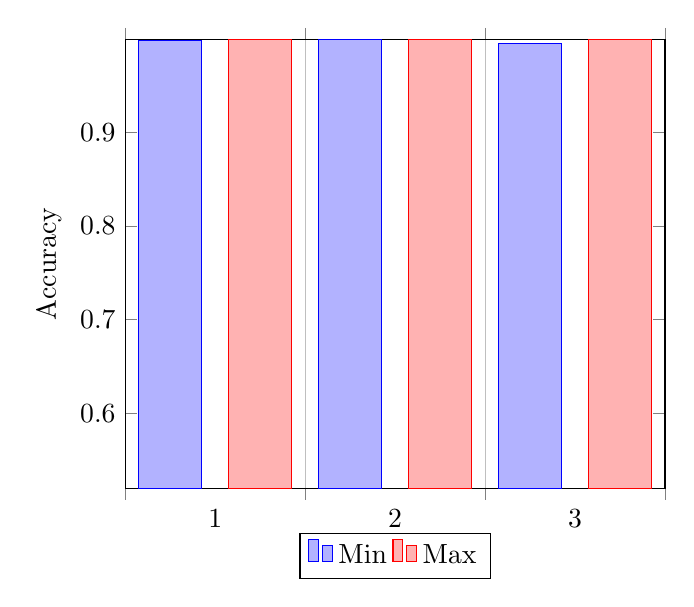
\begin{tikzpicture}
        \begin{axis}[
            x tick label style={
                /pgf/number format/1000 sep=},
            ylabel=Accuracy,
            enlargelimits=0.00001,
            legend style={at={(0.5,-0.1)},
            anchor=north,legend columns=-1},
            ybar interval=0.7,
        ]
        \addplot 
            coordinates {(1, 0.9975) (2, 0.99871) (3, 0.9944) (4, 0.5201)};
        \addplot 
            coordinates {(1, 0.9987) (2, 0.99872) (3, 0.9987) (4, 0.9987)};
        \legend{Min,Max}
        \end{axis}
        \end{tikzpicture}
    \caption{Min-Max accuracy for each fairness algorithm}
\end{figure}

There are some considerations that can be made about the accurencies presented:
\begin{enumerate}

    \item \emph{Maximum Variance with Grid Search:} The algorithm that demonstrates the maximum variance in accuracy results for both the XGB and RF models is Grid Search (GS). This indicates that GS is robust in yielding consistent accuracy outcomes, showcasing its stability in diverse scenarios.

    \item \emph{Minimum Variance with Fairness through Unawareness:} In contrast, the Fairness through Unawareness (FtU) algorithm exhibits the minmum variance in accuracy values across different configurations. More specifically the accuracy is the same for both models. Furthermore this algorithm has the maximum accuracy, values that it shares with other 2 algorithms (DA and EG), but in contrast with them it has the maximum minimum value. This result suggests to choose FtU as fairness algorithm to achieve the maximum accuracy.
\end{enumerate}

Similarly, for each fairness algorithm, the minimum and maximum fairness values are presented. This evaluation allows for an understanding of the fairness outcomes associated with different algorithms, providing a comprehensive view of the trade-offs between accuracy and fairness.
\newpage
\textbf{Disparate Impact Sex}
\begin{figure}[H]
    \centering
    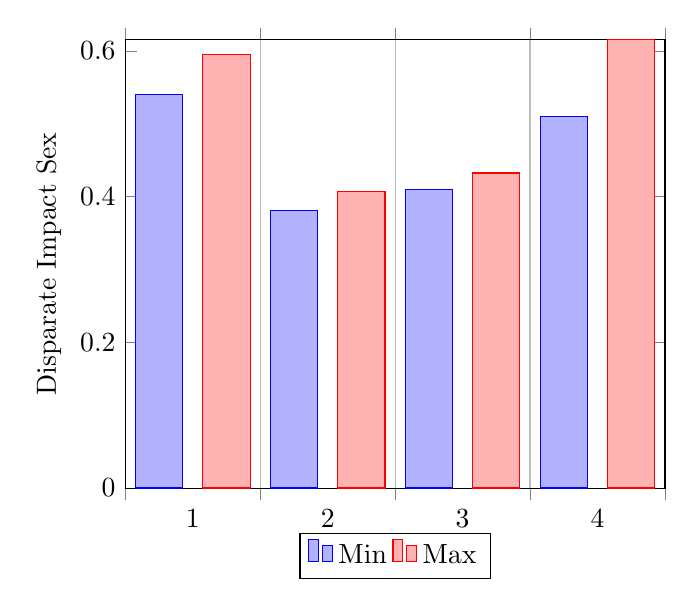
\begin{tikzpicture}
        \begin{axis}[
            x tick label style={
                /pgf/number format/1000 sep=},
            ylabel=Disparate Impact Sex,
            enlargelimits=0.0001,
            legend style={at={(0.5,-0.1)},
            anchor=north,legend columns=-1},
            ybar interval=0.7,
        ]
        \addplot 
            coordinates {(1, 0.5409) (2, 0.3809) (3, 0.4103) (4, 0.5102) (5, 0.0000)};
        \addplot 
            coordinates {(1, 0.5950) (2, 0.4075) (3, 0.4325) (4, 0.6154) (5, 0.0000)};
        \legend{Min,Max}
        \end{axis}
        \end{tikzpicture}
    \caption{Min-Max Disparate Impact Metric for Sex protected attributes and for each fairness algorithm}
\end{figure}

